\documentclass[a4paper]{article}

\usepackage{amsfonts}
\usepackage{a4wide,times}
\usepackage[english]{babel}
\usepackage{graphicx}
\usepackage{listings}
\usepackage[parfill]{parskip}
\lstset{language=Java,
  numberstyle=\footnotesize,
  basicstyle=\footnotesize,
  numbers= left,
  stepnumber=1,
  tabsize=2,
  frame=shadowbox,
  breaklines=true
}


\begin{document}

\title{Net-computing\\
Architectural design document\\
Smart car on demand
}

\date{\today}

\author{Peri Rahamim (s2683423),\\
Jits Schilperoort (s2788659),\\
Twan Schoonen (s2756978)
}


\maketitle
\section*{Project description}
Smart car on demand is the name of our project idea to have self-driving cars drive through the city, and get ordered by costumers who wish to go somewhere using this service. The order is done by a costumer logging in to a mobile application, and select their destination and number of passengers.

The request has the user's location saved, is sent to the car center, that selects the nearest car that can handle the request. Payment is done via money that is saved in the app account (top up is required beforehand). Requests are handled in queue order (first order-first served, maybe we add some priority).

The car arrives to the costumer(s) and takes them to their destination. Selecting a car and planning routes are handled by Artificial Intelligence systems that is able to compute the shortest route. The AI also allows the automated cars to drive without human intervention.

Since this is a big project, we will not implement all of the features, but only those relevant for this course. This list specifies the different elements of the system, with an explanation of why we decided to implement or not implement it:
\begin{itemize}
    \item \textbf{Mobile application:} Each costumer that is interested in getting a car to drive them uses a mobile app to make the order. A working app with an user friendly GUI is irrelevant for this course, so we decided to have a data structure that represents a user and has location, number of people who want to use the service, and destination instead. The mobile app should have money balance of a client included, but we are not implementing this feature because it is irrelevant to this course.
    \begin{itemize}
        \item \textbf{Menus:} The interface of the app is fully text based and operated using the command line. The user gets a menu with the options log in, create a new user, etc. To make a decision, usually a number related to the option has to be entered in the command line. Most decisions open a new menu with new options. Through these menus a user can order a car to its location. 
    \end{itemize}
    \item \textbf{AI:} The automated driving cars should know how to drive on roads without the help of humans. The AI of the car should follow the law and consider other cars (agents) or people crossing the road in its surrounding. This part is obviously too much to implement, and since it is also irrelevant to this course, we decided to assume the AI works. As the AI is implemented, it just follows random patterns around the map and the cars cannot collide with each other or with costumers. 
    \item \textbf{Shortest distance algorithm:} We want the car to find the best route to reach its costumer, considering traffic and other parameters (such as construction that blocks the road). The algorithm helps deciding which car is most suitable to get to a costumer, in case there are more than one car in different parts of the city. To make this work we need live data, so for this project, we only send messages with datasets we made ourselves, and leave out the complicated calculations. The shortest distance is calculated using the Manhattan distance.
    \item \textbf{City layout:} To represent a city, we use a 796x600 image that contains rectangles representing buildings. Coordinates are represented as numbers 0-8 in the x axis and 0-6 in the y axis. Each frame retrieves locations of clients (marked as red points) and cars (marked as blue points). A city is represented in the menu as a center, we can have a maximum of 9 centers, each with its own color. To go from a city map to centers menu, press 'b'.
    \item \textbf{Order handling:} The cars' and costumers' locations are changed according to order handling in the following way: when a client sends an order, they wait for an available car. When there is a car assigned to the costumer, the costumer's location is shown on the map according to the coordinates of their location along with their final destination. The available car with the shortest distance to the client goes to pick up the client, and changes its $isAvailable$ Boolean to False (initialized as True). When costumers are picked up, they no longer appear on the map. The car, along with the costumer who is no longer represented on the map, goes to the client's destination, that also disappears when the car arrives. The program only handles location and destination in the same center. In case the destination belongs to a different center from where the car came from, the origin center and the destination center should update their cars lists, by removing the car from origin center's list, and adding it to new center's list, however for lack of time we did not implement this feature. After arriving to the client's destination, the Boolean $isAvailable$ is changed to True, and the car returns to its (origin/new) center.
\end{itemize}

\section*{Project requirements}
The requirements that are implemented in this project are listed as follows:
\begin{itemize}
    \item \textbf{Socket:} used for center to car and costumer to center communication.
    \item \textbf{Message queuing:} the requests made by the mobile application are queued by the centers, when there are available cars, the center dequeues the order and asigns it to a car. 
    \item \textbf{Web services (REST):} the mobile app communicates with the database by using REST. This is used for getting client's information.
\end{itemize}

\subsection*{Star vs P2P topology}
\textbf{Star topology:} The star topology is used by the centers to control the cars. Here the cars only drive and all computing is done by the center.\\
\textbf{P2P topology:} This method was planned to be used for center to center communication, so when a car leaves the district or city, the centers communicate with each other and update cars lists. Eventually, we decided not to implement it since we don't have the time to test it.

\section*{Program design}
To complete this project, we decided to use the language Python. The reason behind this decision is that Python includes countless libraries to help programmers deliver products without the need to worry about writing algorithms that take care of basic functionality. More specifically, our program includes the following libraries:
\begin{itemize}
	\item \textbf{socket:} used for sending socket messages.
	\item \textbf{threading:} for handling sockets.
	\item \textbf{pika:} used for message queuing.
	\item \textbf{flask:} for REST.
	\item \textbf{flast\_httpauth:} for authentication.
	\item \textbf{flask\_sqlalchemy:} for database.
	\item \textbf{passlib.apps:} for password hashing.
	\item \textbf{pygame:} for graphical representation of the project.
\end{itemize}
\\The way our project is designed, four scripts are used, these scripts are communicating with each other using networking. 
\begin{enumerate}
    \item The first script is the REST app (path: src/RestApp/restapp.py), that is used as the server for client management. It uses database and authentication, and stores only password hashes. However, authentication requests are done in plain text, making the connection not entirely secured. This script runs on port 5000 on localhost unless an argument is added when running the script, then the script runs on address 0.0.0.
    \item The second script is the (mobile) application (path: src/App/app.py). It uses the command line to interact with the user, this could be done with comfortable GUI, however it would be time consuming and irrelevant for the purpose of this project. It interacts with the REST server, it assumes to be running on localhost, if the user wishes to change this, option 3 in main menu should be chosen. After user management is done and they are logged in, and an order is sent, the script uses rabbitmq to send a message to the correct center. Rabbitmq is also assumed to be running on localhost, if the user wants this to be changed, an argument should be added to the script specifying the ip address. This message is not durable, so if there is no center running with the name that was entered in the order, the message is lost. Note that when an order is sent, the order requests for number of passengers and center destination, these variables are not used.
    \item The third script is center (path: src/App/center.py). Initially, the script asks for a center's name, number of cars in the center, and a port number. The port number is used for the cars connecting to the server. First, the center starts its own server, used for listening to new cars, then it sends a UDP message to the map, specifying that the center exists, how many cars it has, its address, and its port (note that this port should be free, so ports 5000, 1234 should not be chosen). This is done on localhost port 1234 and is not configurable, this means the center and the map should be running on the same computer. This decision was made since we wanted to have some sort of representation for cars, we chose to have it using a map. The UDP protocol is chosen for two reasons, first, when running on localhost packages are not lost, second, we wanted to have a center running even when the map is not running, that would be impossible if we used TCP protocol.
    \item The fourth script is mapapp (path: src/MapApp/mapapp.py), this script is used for creating map with cars, it has its own UDP server listening to events in case it receives a request to add centers, cars, or costumers. Once a request from a server to add cars is received, the cars are created, and every car gets its own client connected using TCP, to the center they belong to. These cars are saved in the center's server and their state is remembered for car-center communication. The car-center communication from here on is not dependant on the map, since the map only listens to events and has no control over the cars.
\end{enumerate}


\section*{Component diagram}
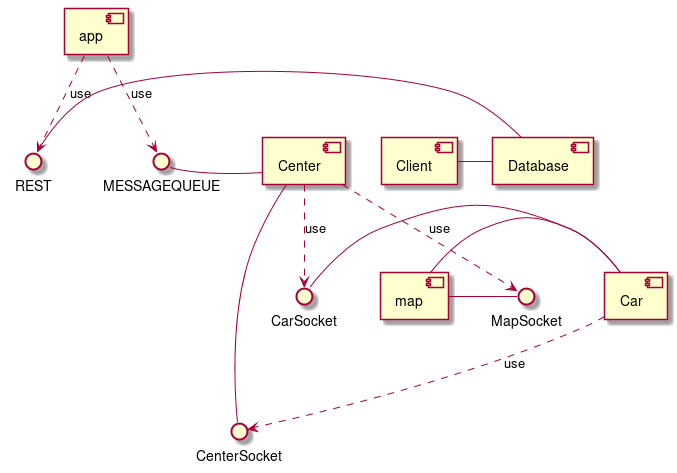
\includegraphics[width=1\textwidth]{../Diagrams/componentDiagram.png}

\section*{Class diagram}
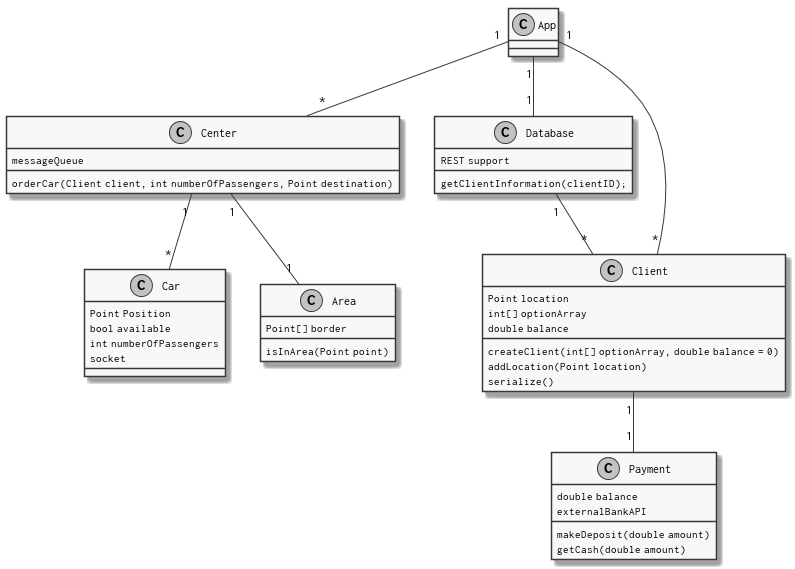
\includegraphics[width=1\textwidth]{../Diagrams/classDiagram.png}

\section*{Sequence diagrams}
\subsection*{RegisterClient}
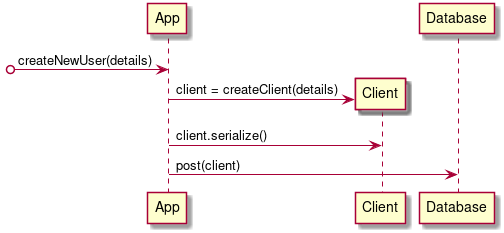
\includegraphics[width=1\textwidth]{../Diagrams/registerClient.png}\\
The client requests to sign up. App creates new object Client with the client's data that contains their personal preferences and money balance in the account. Client object is serialized and put in the database.

\subsection*{OrderCar}
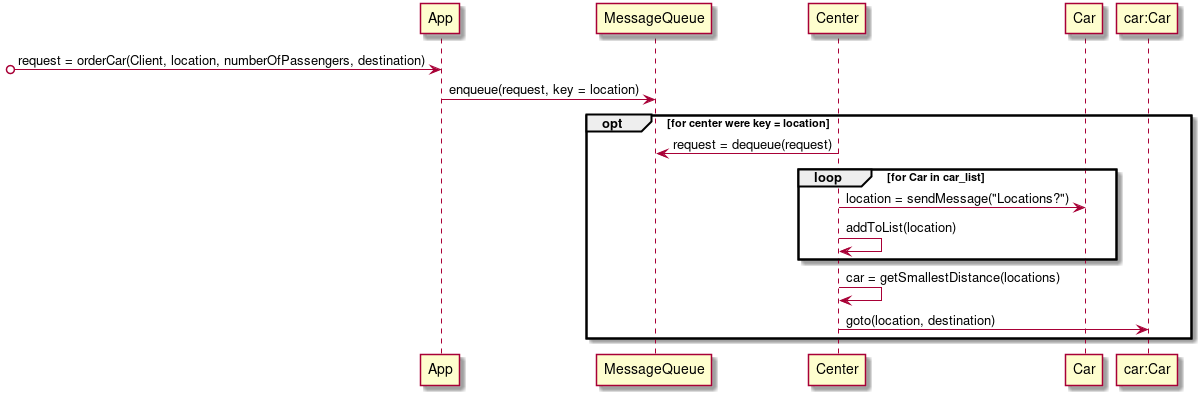
\includegraphics[width=1\textwidth]{../Diagrams/orderCar.png}\\
When a costumer orders a car, the app first checks in which area the costumer is, to know to which center it should send the order. The app then sends the order that has the object Client, the number of passengers, and the destination to the center. The center enqueues the order.
\subsection*{SendCar}
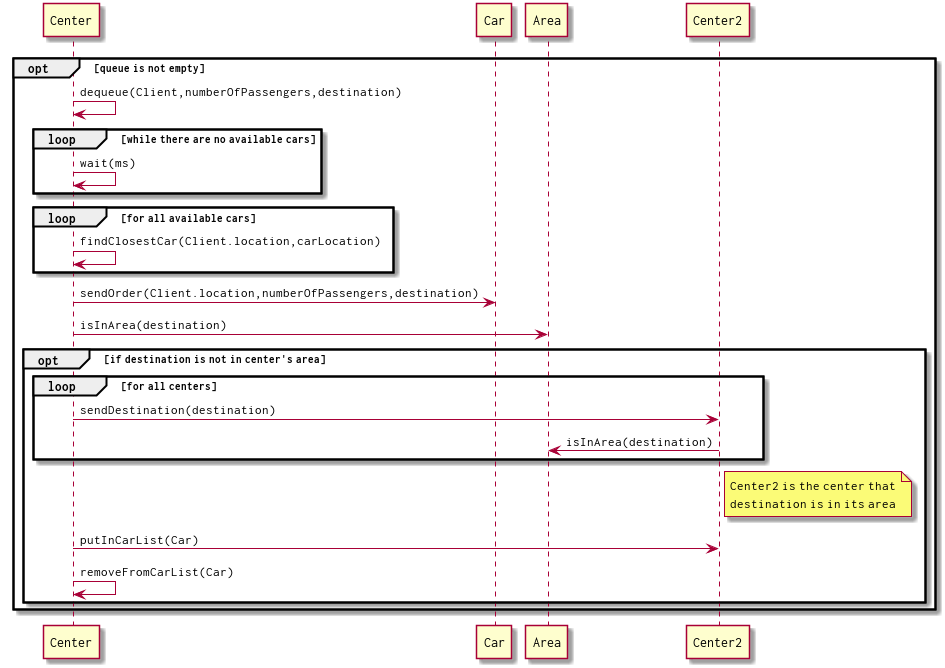
\includegraphics[width=1\textwidth]{../Diagrams/sendCar.png}\\
The entire use case starts only if queue is not empty. Center dequeues order. If there are no available cars, the center waits, and after this loop is terminated, it looks over the list of available cars, and finds the available car that is the closest to the client's location. The center sends the order to the car it found. The center checks if the destination is in its area, if not, the center sends the destination to all centers to check which one covers the area, and the car is removed from the list of the first center and entered to the list of the second center. 

\end{document}
